\documentclass{beamer}
%\usetheme{AnnArbor}
\usetheme{Goettingen}
\usecolortheme{orchid}
\usepackage{hyperref}

% Title page details:
\title{Locks in SMB/Samba}
\author{Michael Adam (\href{mailto:obnox@samba.org}{obnox@samba.org})}

%%\date{\today}
\date{November 6, 2025}

\begin{document}
\setbeamercovered{transparent}

\begin{frame}
    \titlepage
\end{frame}



%% outline at start of each section:
%% https://statisticaloddsandends.wordpress.com/2019/02/18/beamer-inserting-section-slides-before-each-section/

\AtBeginSection[]
{
    \begin{frame}
        \frametitle{Outline}
        \tableofcontents[hideallsubsections,currentsection]
    \end{frame}
}


\section<presentation>[outline]{Outline}
%%\begin{frame}{Outline}
%%\tableofcontents[currentsection]
%%\end{frame}

%% trick to also hide first toc-item:
%% https://tex.stackexchange.com/questions/298647/beamer-table-of-contents-with-first-section-shaded
%\begin{frame}{Outline}
%\tableofcontents[hideallsubsections,sectionstyle=shaded]
%\end{frame}
%\addtocounter{framenumber}{-1}
%\begin{frame}{Outline}
%\tableofcontents[hideallsubsections,pausesections]
%\end{frame}

\section<presentation>[start]{Opening}
\begin{frame}{The Start}
\begin{block}{Talking about...}<2->
    Locking concepts in SMB
\end{block}
\end{frame}


\begin{frame}{Why locks?}
    \includegraphics[width=\paperwidth,height=\paperheight,keepaspectratio]{lock.jpg}
\end{frame}

\section<presentation>[concepts]{SMB locking concepts}
\begin{frame}{SMB locking concepts}
\pause
\begin{itemize}[<+->]
\item share modes - whole file locks
\item byte range locks (brlocks)
\item oplocks/leases
\end{itemize}
\end{frame}


\section<presentation>[SMB vs POSIX]{SMB vs POSIX, conceptually}
\begin{frame}{SMB vs POSIX, conceptually}
    \pause
\begin{itemize}[<+->]
\item SMB: mandatory/enforced
\item POSIX: advisory/voluntary
\end{itemize}
\end{frame}

\section<presentation>[share modes]{share modes}
\begin{frame}{share modes}
    \pause
\begin{itemize}[<+->]
\item like locks of entire files
\item  acquired at open/create (share access)
\item allow/deny concurrent opens with certain access modes
     \pause
     \begin{itemize}[<+->]
     \item share read
     \item share write
     \item share delete
     \end{itemize}
\end{itemize}
\end{frame}



\section<presentation>[brlocks]{byte range locks(brlocks)}
\begin{frame}{byte range locks (brlocks)}
\pause
\begin{itemize}[<+->]
\item lock parts of files (example: spreadsheet cells/database records)
\item separate LOCK call
\end{itemize}
\end{frame}


\section<presentation>[oplocks/leases]{oplocks/leases}
\begin{frame}{oplocks/leases}
\begin{block}{Entering}
 oplocks and leases...
\end{block}
\end{frame}
\subsection{oplocks/leases - concepts}
\begin{frame}{oplocks/leases - concepts}
\begin{block}{oplocks (opportunistic locks)}<2->
\begin{itemize}
\item \textbf{not actually locks!}
\item client-side caching (reads, writes, brlocks ..)
\item requested/granted at open/CREATE
\item "broken" by second open
\end{itemize}
\end{block}
\begin{block}{oplock benefits}<3->
    \begin{itemize}
    \item reduce network traffic
    \item $\Rightarrow$ better file sharing  performance
    \end{itemize}
\end{block}
\begin{block}{leases / lease oplocks}<4->
\begin{itemize}
\item from SMB 2.1+
\item enhanced/improved  oplocks
\item lease key $\Rightarrow$ multiple opens per client

 \item requested via oplock level lease
\end{itemize}
\end{block}
\begin{block}{oplocks: relevance}<5->
    \begin{itemize}
    \item mostly SMB1
    \item still exist in SMB3
    \item effectively superseded by leases
    \end{itemize}
\end{block}
\end{frame}
\subsection{oplock levels and lease types}
\begin{frame}{oplock levels and lease types}
\begin{block}{oplock levels}<2->
\begin{itemize}
    \item level 1 (exclusive)
    \item level 2 (shared)
    \item batch
    \item lease
\end{itemize}
\end{block}

\begin{block}{lease types}<3->
\begin{itemize}
\item R: read caching
\item W: write caching
\item H: handle caching
\item RH: combined read and handle caching
\item RW: ...
\item RWH: ...
\end{itemize}
\end{block}
\end{frame}


\subsection{oplocks/leases - mapping}
\begin{frame}{oplocks/leases - mapping}
\begin{block}{rough correspondence}<2->
    \begin{center}
    \begin{tabular}{ |c|c| }
    \hline
    oplock lvl & lease type \\
    level 1 & RW \\
    level 2 & R \\
    batch & RW \\
    \hline
    \end{tabular}
\end{center}
\end{block}

\begin{alertblock}{warning}<3->
  \textbf{ this is rather coarse -- details differ!}
\end{alertblock}
\begin{alertblock}{Relevance}<4->
\textbf{SMB1 vs SMB3}
\end{alertblock}
\end{frame}

\subsection{oplocks/leases - references}
\begin{frame}{oplocks/leases - references}
\begin{block}{MS oplock doc}<2->
\url{https://learn.microsoft.com/en-us/windows/win32/fileio/types-of-opportunistic-locks}
\end{block}
\begin{block}{MS breaking oplocks}<3->
\url{https://learn.microsoft.com/en-us/windows/win32/fileio/breaking-opportunistic-locks}
\end{block}
\begin{block}{excellent (German!) article about SMB 2.2, oplocks, and leases by Volker}<4->
\url{https://www.heise.de/ratgeber/Version-2-2-des-SMB-Protokolls-1703492.html?seite=2}
\end{block}
\end{frame}

\section<presentation>[SMB2 CREATE]{The SMB2 CREATE call}
\begin{frame}{The SMB2 CREATE call}
\begin{block}{a pretty complicated/complex call}<2->
        It does many things:
\begin{itemize}
\item open existing  files
\item create new files
\item oplocks/leases
\item share modes
\end{itemize}
\end{block}

\begin{block}{important fields}<3->
    \begin{itemize}
    \item filename
    \item CreateDisposition:
    \begin{itemize}
       \item open existing files
       \item create new files
    \end{itemize}
    \item FileAttributes: for creating new
\item CreateAttributes:  e. g. for directories
    \item DesiredAccess
    \item ShareAccess: share modes
    \item RequestedOplockLevel
    \item list of create contexts (e. g. for leases)
    \end{itemize}
\end{block}
\end{frame}

\begin{frame}{create spec docs}
\begin{block}{MS protocol spec SMB2 CREATE REQUEST}
    \url{https://learn.microsoft.com/en-us/openspecs/windows_protocols/ms-smb2/e8fb45c1-a03d-44ca-b7ae-47385cfd7997}
\end{block}
\begin{block}{MS protocol spec  SMB2\_CREATE\_LEASE context}
\url{https://learn.microsoft.com/en-us/openspecs/windows_protocols/ms-smb2/250a5100-f8b0-4b32-a202-f592ce4c05e7}
\end{block}
\end{frame}

\section<presentation>[mappings]{Correspondences and Mappings}
\begin{frame}{correspondence SMB$\leftrightarrow$ POSIX}
\begin{block}{correspondence}<2->
\begin{center}
\begin{tabular}{ |c|c| }
\hline
SMB & POSIX \\
share mode & flock \\
brlock & fcntl brlock \\
oplock/lease & Linux kernel oplock \\
\hline
\end{tabular}
\end{center}
\end{block}
\begin{alertblock}{warning}<3->
  \textbf{ this is rather coarse -- details differ!}
\end{alertblock}
\end{frame}




\begin{frame}{samba mapping options}
\begin{block}{\texttt{smb.conf} options}<2->
\begin{itemize}
\item \texttt{posix locking}
\item \texttt{kernel share modes}
\item \texttt{kernel oplocks} (Linux only)
\end{itemize}
\end{block}
\end{frame}


\section<presentation>[references]{general SMB References}
\begin{frame}{general references}
\begin{block}{overview:File sharing with SMB(3)}<2->
\url{https://learn.microsoft.com/en-us/windows-server/storage/file-server/file-server-smb-overview}
\end{block}
\begin{block}{MSSMB protocol docs}<3->
\url{https://learn.microsoft.com/en-us/openspecs/windows_protocols/ms-smb/f210069c-7086-4dc2-885e-861d837df688}
\end{block}
\end{frame}



\section<presentation>[multi-proto]{ Multi-protocol}
\begin{frame}{What about Multi-Protocol?}
\begin{block}{yeah, what about it?}
\begin{itemize}
\item POSIX: see above
\item NFS: see below
\item S3: not here ...
\end{itemize}
\end{block}
\end{frame}

\begin{frame}{Multi-Proto: SMB $\leftrightarrow$ NFS}
\begin{block}{SMB $\leftrightarrow$ NFS}<2->
\begin{center}
\begin{tabular}{ |c|c| }
\hline
 SMB3 & NFS4  \\
 lease & delegation \\
 share mode & share reservation \\
 other & client request \\
\hline
\end{tabular}
\end{center}
\end{block}
\begin{alertblock}{Warning}<3->

\textbf{cum grano salis -- details differ}
\end{alertblock}
\begin{alertblock}{TODO: Multi-Protocol}<4->
\begin{itemize}
\item Ganesha+CephFS has clustered delegations and reservations.
\item Correct? ($\Rightarrow$ verify!)
\item via FSAL? ($\Rightarrow$ verify!)
\item: how do they do it? $\Rightarrow$ A model for Samba? ($\Rightarrow$ try!)
\end{itemize}
\end{alertblock}
\end{frame}

    \section<presentation>[end]{Wrap-up}
\begin{frame}{The End}
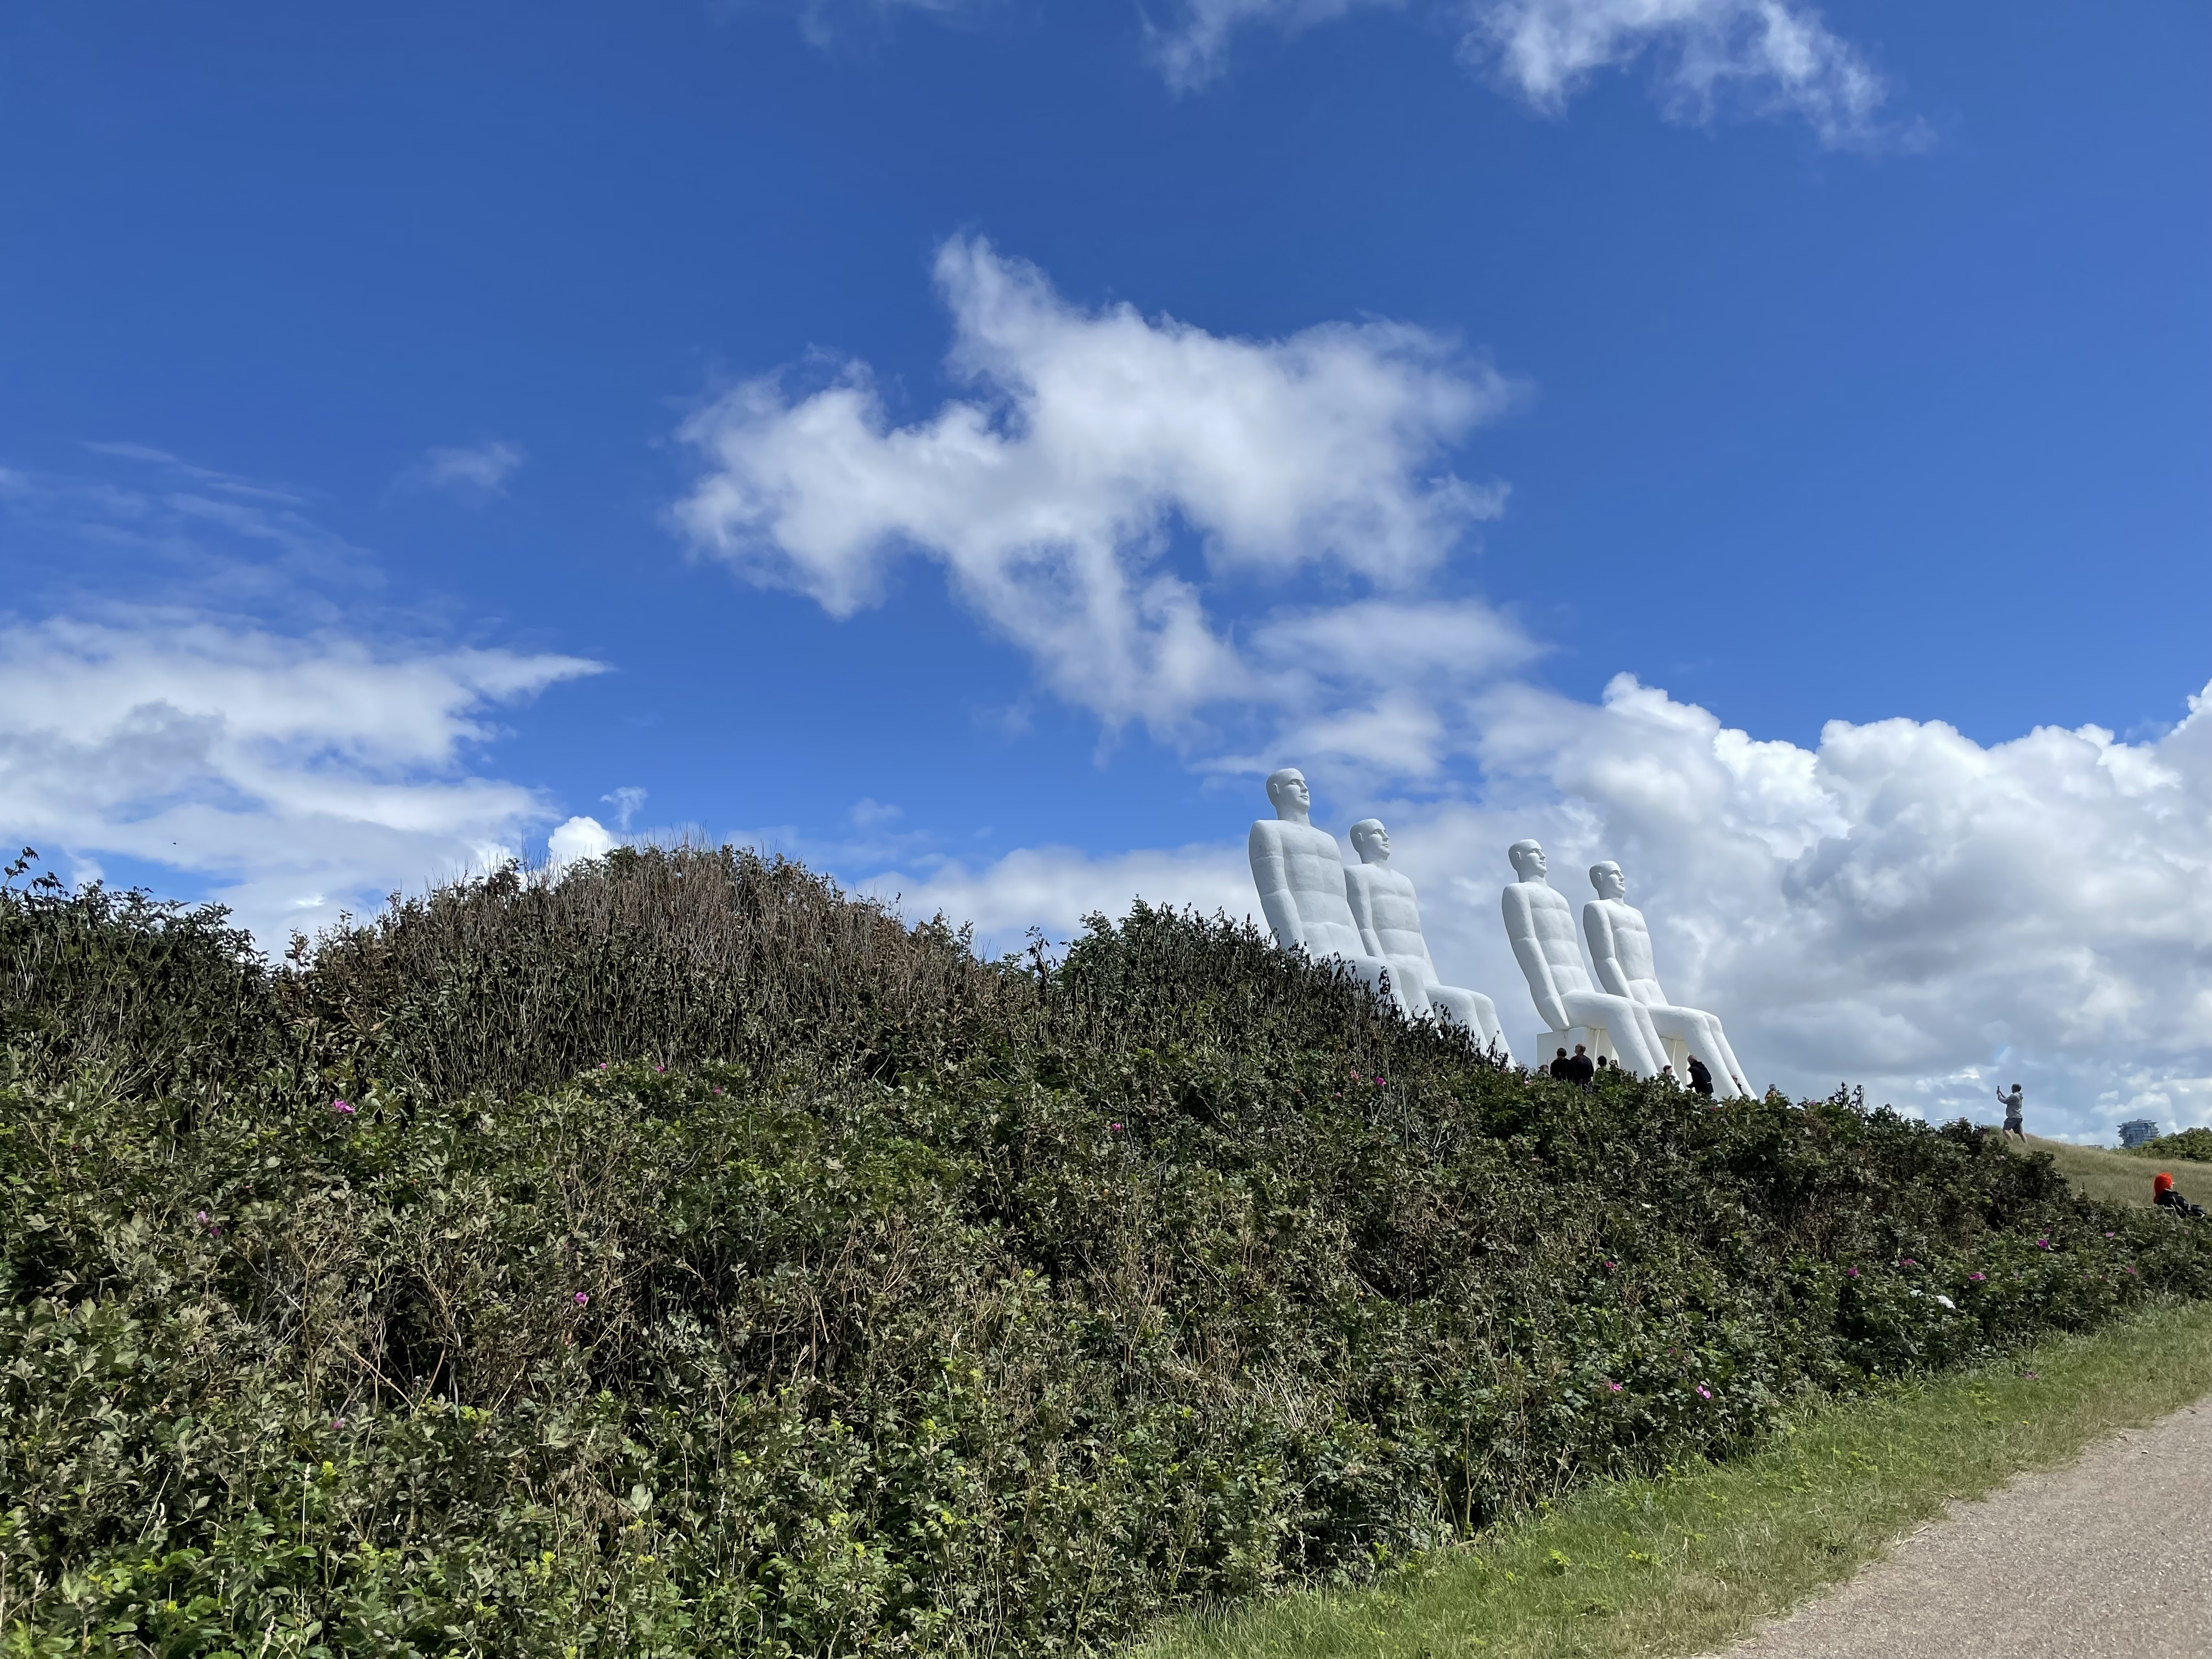
\includegraphics[width=\paperwidth,height=\paperheight,keepaspectratio]{mennesket_og_havet.jpg}
\end{frame}

\begin{frame}{The End}
\begin{block}{That's it}<2->
    For now...
\end{block}
\begin{block}{Questions?}<3->
Discussion ...
\end{block}
\end{frame}




\end{document}


